\documentclass[../main.tex]{subfiles}

\begin{document}

In this chapter we introduce the main contribution of this thesis, we describe the proposed design flow and how it is implemented as part of the Halide infrastructure. 
In section \ref{motivations} we describe the motivations to use HLS tools to deploy DL models on FPGAs. We describe the main HW platform that can be used to perform inference and their drawbacks. 
In section \ref{back-end} we describe how the Bambu back-end works and how it is implemented inside the Halide infrastructure. We describe the main steps and possible future improvements.
\newpage

\section{Motivations}
\label {motivations}
Since the state of the art DL models are becoming increasingly more complex and demanding in terms of computational power, using CPUs and GPGPUs as inference platforms is becoming a less appealing approach. 
When a model is deployed the system is required to satisfy latency, throughput and memory consumption constraints; CPUs are not suitable for high throughput applications and power hungry GPUs have high latency due to memory transfers between host and accelerator.
The use specialized ASICs meet all 3 requirements with high throughput, low latency and memory consumption; but such a solution is not flexible and not able to express new layers that might have not been yet invented.

A different approach is to use Field Programmable Gate Arrays (FPGA); the use of programmable HW allow the possibility to satisfy all system requirements while being able to use the system to deploy different models.
The problem with FPGAs is the time required to deploy an FPGA's application; deploying a correct and optimized bitstream is not trivial and require a long design time. To reduce that problem High Level Synthesis tools are used; these tools take as input the abstract representation of a program, in this case a DL models, and produce as output the optimized bitstream to be deployed. The final result do not have the same performance that a manually designed and optimized solution would have but allow fast prototyping and the use of FPGAs to deploy models without the need of being an expert of the design process.

The integration of a Bambu back-end in Halide allow the programmer to easily deploy a DL model on FPGA; the decoupling of the schedule from the algorithm definition allow the programmer to leverage the possibility to deploy multiple models in a short amount of time and find the schedule that better fit the target architecture and memory hierarchy.

\newpage

\section{Design flow}
\label {design-flow}
The goal of the proposed design flow is to leverage PandA - bambu and the Halide infrastructure to deploy a Deep Learning model on FPGA while being able to optimize the sequence of scheduled operations for the target architecture.


\begin{figure}[h!]
  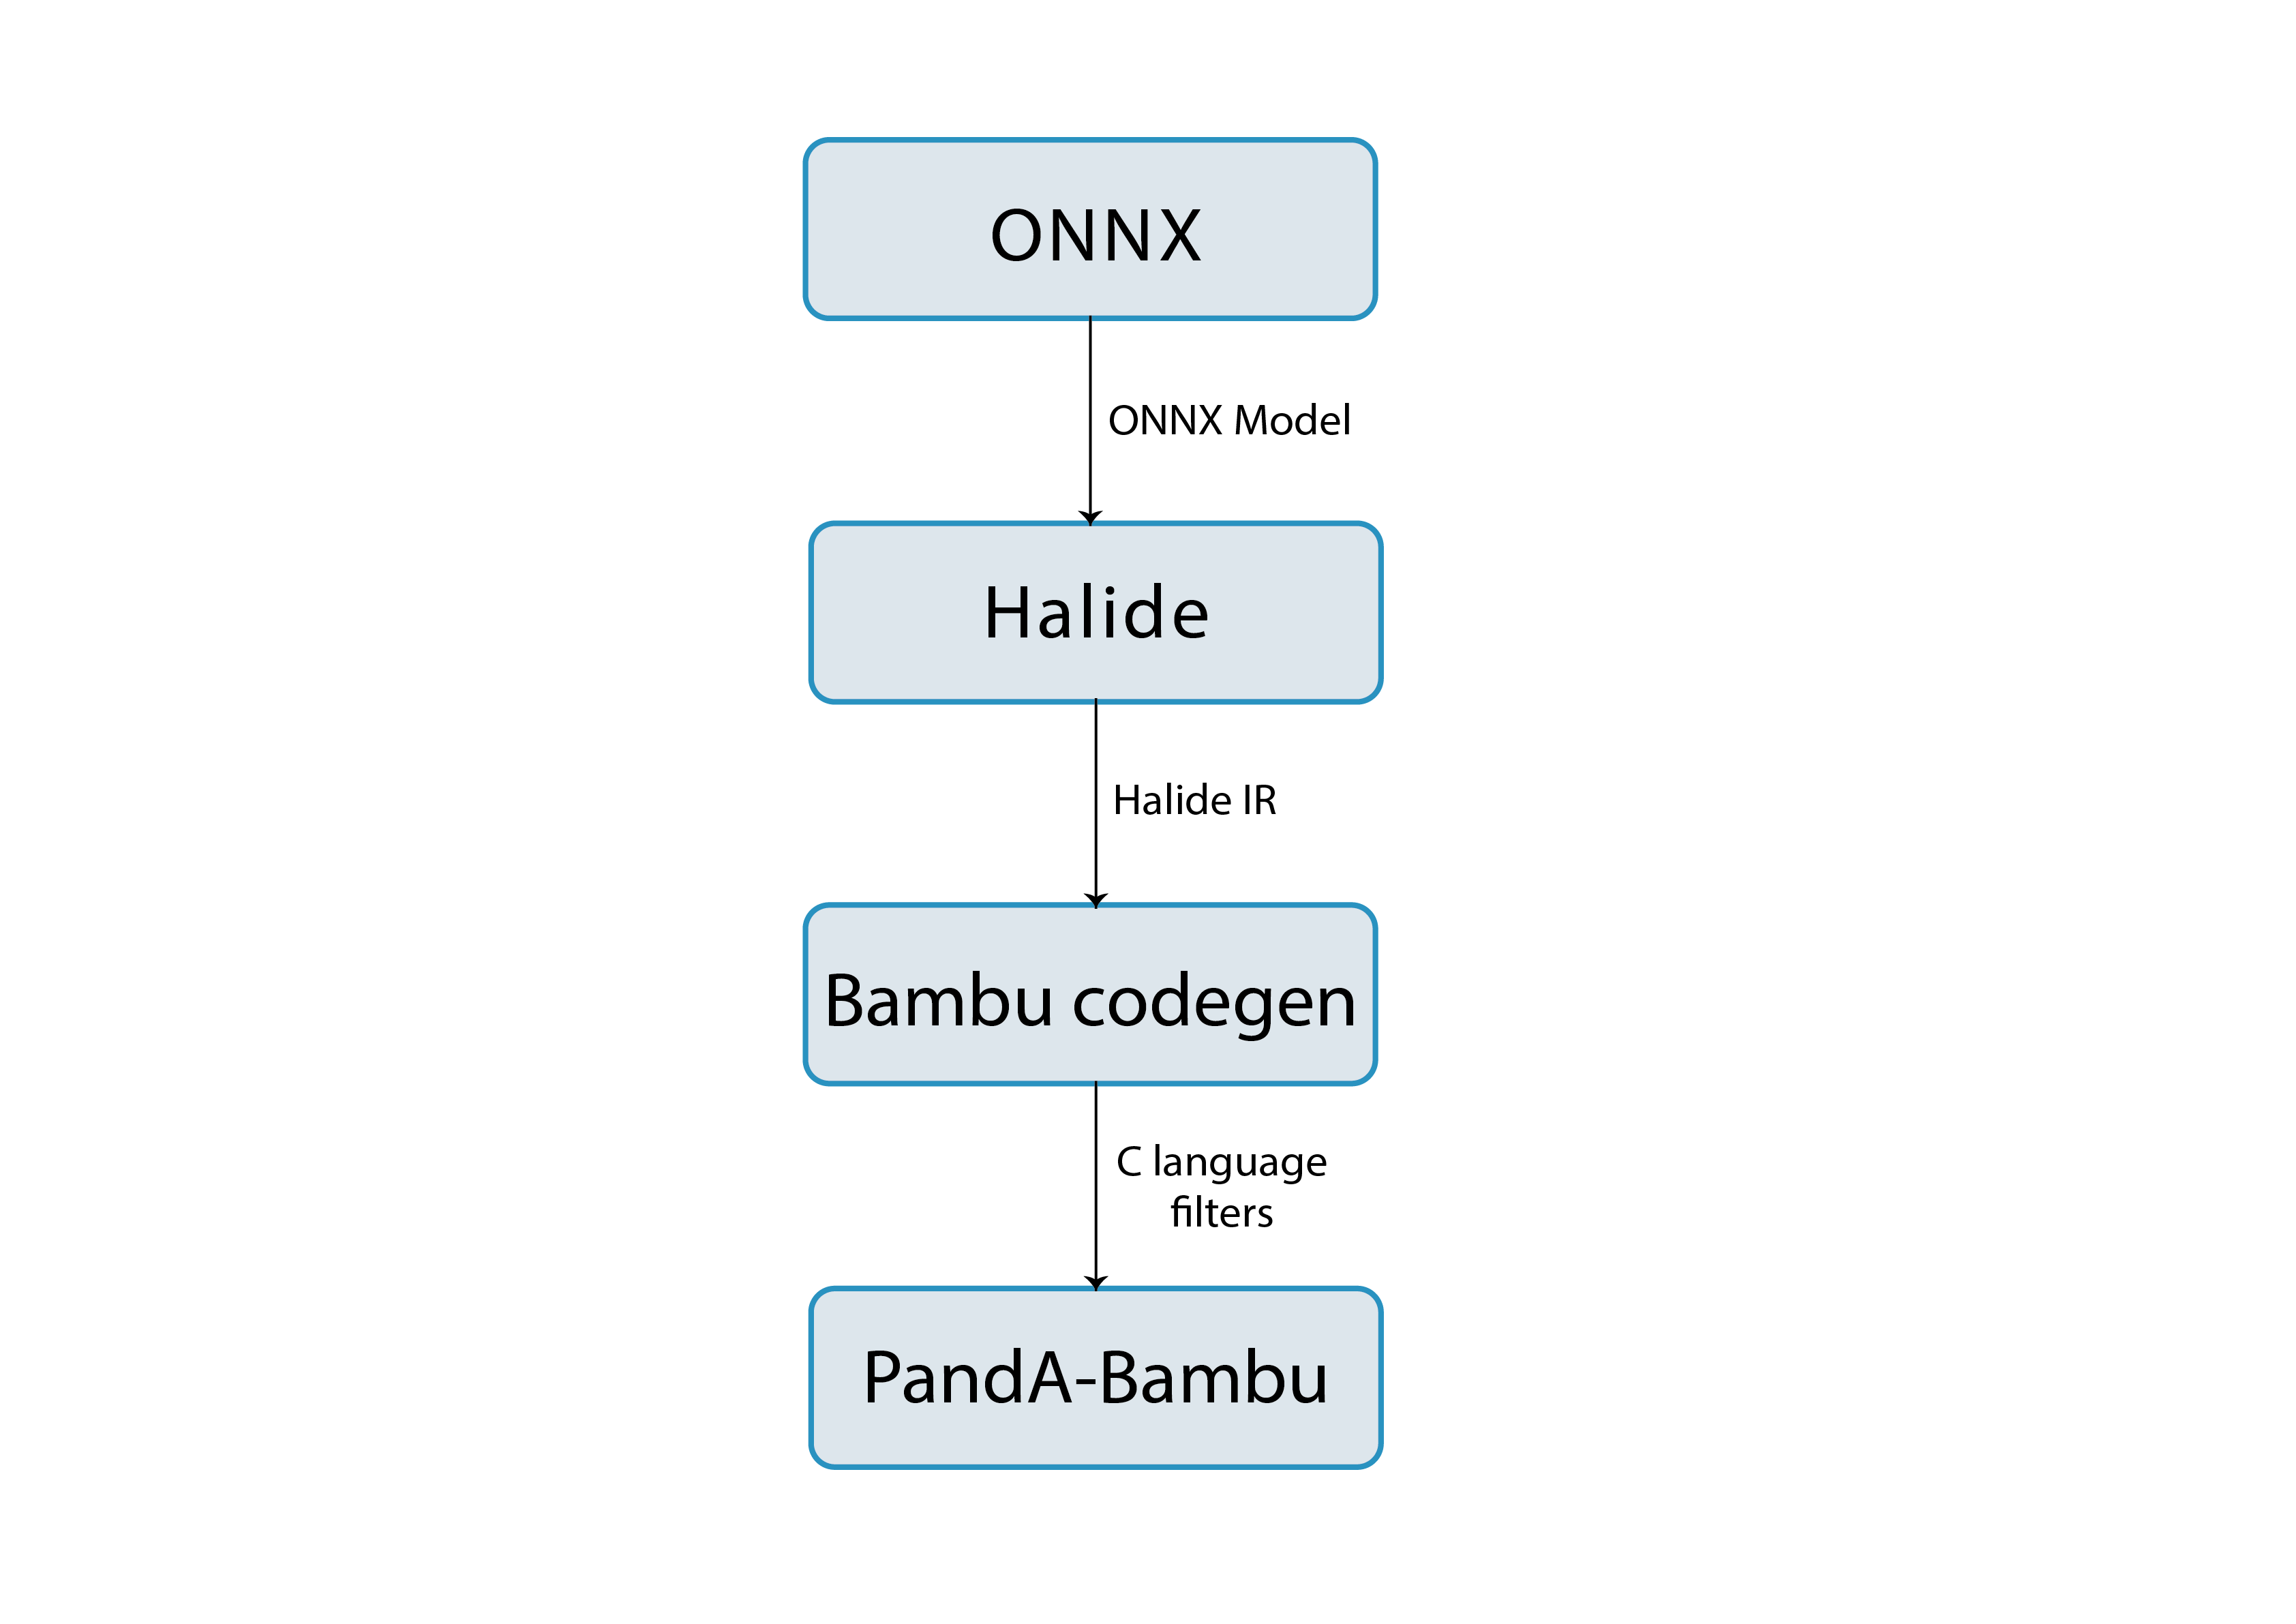
\includegraphics[width=1\textwidth]{images/Stack.png}
  \centering
  \caption{Design Flow}
  \label{fig:DesignFlowStack}
\end{figure}

\bigskip
The starting point is a Deep Neural Network model provided from one of the most common frameworks. Since each framework represent the computational graph in different ways we to use a common representation to provide a unique entry point to the proposed design flow. The Open Neural Network eXchange specification (ONNX) has been used as common representation; using ONNX allows the portability of computational graphs between different frameworks and is already supported by the Halide infrastructure.

To increase the performance of a forward pass of a DL models the design flow incorporate two optional steps: By using the VitisAI tools the programmer can perform pruning and quantization on the ONNX model. The pruning optimization increase the performance of the final model by reducing the amount of work that has to be done by removing the less useful connections between neurons and the quantization reduce the floating point precision of the operations. The latter is especially useful for FPGAs since the floating point precision can be easily adapted. 

Given the ONNX model that need to be deployed the Halide framework have a built-in tool to convert it to a internal generator. The programmer can then decide how to schedule the imported model by defining the schedule method of the generator, as for any other algorithm. 

Halide can then proceed by converting the scheduled generator to a internal IR before feeding the optimized representation to the Bambu back-end that has been developed to provide support for FPGA targets.


\section{The Bambu back-end}
\label {back-end}
To implement a new back-end the Halide infrastructure allow the creation of target specific codegens that take as input the Halide IR and produce the final optimized code. Each target architecture have it's own back-end, that allow the Halide infrastructure to take advantage of architecture specific features and optimizations.

The Bambu back-end take as input the Halide IR and produce the C code to be used within the bambu framework. The code generation is split in 3 main steps: Filters extraction, IR optimizations and code generation. In the next sections describe the three steps in details.

\subsection{Filters extraction}
The filters extraction step take as input the Halide IR and produce a DAG representation of the Halide lowered function. 
The DAG is composed by interconnected filters related by a producer consumer relationship. 
Such relationship is already extracted by the Halide infrastructure and can be easily extracted by leveraging the ProducerConsumer statement of the Halide IR.

\newpage
\begin{lstlisting}[caption= Example of filter extracted from the Halide IR. The extracted code is hard to translate to c language and access the memory buffers at each iteration. ]
X_im_padded_U_sum_3[0] = 0.000000f
for (x_7, 0, 3) {
    for (x_8, 0, 3) {
        X_im_padded_U_sum_3[0] = ((float32)X_im_padded_U_sum_3[0] 
          + ((float32)b2[((x_7*6) x_3)]
          * ((float32)b2[((x_8*6) + x_4)]
          * (float32)b0[((((x_2*3) + x_8)*3) + x_7)])))
    }
}
\end{lstlisting}

Before proceding with the extraction of the DAG filters the codegen clean the IR representation by removing unused constructs, renaming variables and buffers to avoid name conflicts and by substituting into the IR values that are already known at compile time such as the dimensions of the input and output tensors. 
This improves the bound inference analysis of the Halide compiler by reducing the number of variables and increasing the number of fixed size loops inside the Halide IR. 

Once the IR has been preprocessed the producer consumer filters can be extracted.
Each filter of the DAG representation is going to be fully described by the IR code of the filter and the connections with other filters.
Other information about buffers and variables usage are stored in order to make easier the work of subsequent steps.

When the schedule store multiple functions at root granularity the resulting DAG have multiple filters without incoming dependencies. 
This introduce a entry point problem when trying to generate the final code. 
To solve such problem a new base filter is always introduced; the bambu\_main\_filter work as entry point for the computation and is used to store the necessary buffers and call the filters with root store granularity.

\subsection{IR optimizations}
Once the filters has been extracted the program has been represented as a set of interconnected independent filters related by producer consumer relationships. Each filter have its own independent code represented as a Halide statement. The IR code of each filter can be optimized by performing a set of basic optimization passes over the IR code representation such as reducing as much as possible redundant memory accesses and by avoiding recomputation of data shared by different iterations.

The first operation that is performed is the IR preparation for subsequent optimization passes. Each IR operation is split into multiple statements that perform basic operations such as single operators and call to external functions.
Such operation also improve the readability of the generated code.

The first optimization pass performed is pushing each store as outside as possible of the loop nest. This is performed by computing for each store the dependency on other variables and by pushing an operation outside a for loop only if the operation do not depend on the variable of the loop. This allow the final code to avoid recomputation of data shared among different iterations inside the filter execution.
The second optimization pass performed is the fix of multiple read writes on the same buffer inside the filter code. The Halide IR represent the computation by operating directly on the buffer memory. This is not an optimized approach for the code to be generated. When a filter code access a buffer location on the same index inside the same loop the IR is optimized by pushing as outside as possible the read and write memory access inside the IR. The previous memory operations are replaced with access to local variables. 

\newpage
\begin{lstlisting}[caption = Example of optimized IR. The complex operation of the previous example has been split into simple operations. Intermediate results that are shared among different iterations and memory accesses has been pushed outside]
X_im_padded_U_sum_3[0] = 0.000000f
_9[0] = (x_2*3)
_17[0] = (float32)X_im_padded_U_sum_3[0]
for (x_7, 0, 3) {
    _3[0] = (x_7*6)
    _4[0] = (_3 + x_3)
    for (x_8, 0, 3) {
        _6[0] = (x_8*6)
        _7[0] = (_6 + x_4)
        _10[0] = (_9 + x_8)
        _11[0] = (_10*3)
        _12[0] = (_11 + x_7)
        _2[0] = (float32)_17
        _5[0] = (float32)b2[_4]
        _8[0] = (float32)b2[_7]
        _13[0] = (float32)b0[_12]
        _14[0] = ((float32)_8*(float32)_13)
        _15[0] = ((float32)_5*(float32)_14)
        _16[0] = ((float32)_2 + (float32)_15)
        _17[0] = (float32)_16
    }
}
\end{lstlisting}

\bigskip

A third optimization pass is the elimination of trivial buffers of size of one element. When a filter operate on a buffer of single size the buffer is replaced with a variable and is passed to the called filter as a single variable. When the buffer with a size of one element is instead the output buffer the filter return the computed value as the return value of the function representing the filter execution.

An other important optimization is the detection of situations when producer consumer operations allow the usage of FIFO queues to send data between filters. 
If such a situation holds, the memory access on a buffer can be replaced with a FIFO queue. 
FIFO queues are already implemented and optimized inside the Bambu framework; using such a communication channel can improve the memory management of processed values among filters.
At the moment FIFO queues are detected in the trivial case of single read and write accesses on matching indexes and loop nests. 
A future work might improve the detection of FIFO channel by detecting sliding window optimizations 

Once the IR optimization passes has been performed on all filters the DAG is ready to be translated into the C function to be feed to the Bambu framework.

\subsection{Code generation}
After the optimization step the codegen is ready to produce the final code to be used with the Bambu framework. The work is carried out by simply visiting the IR and translating line by line the IR operations to corresponding C operations. To avoid loss of floating point precision when writing constants we decided to write the value of each constant as hexfloat values.

\begin{lstlisting}[caption = Output C code of the example filter. The Halide IR has been translated to C code and encapsulated. Since the filter compute only one value a return statement has been added at the end of the function.]
float X_im_padded_U_sum_3_fun_0(float b0[18], float b2[18],
        int x_2, int x_3, int x_4){
    float X_im_padded_U_sum_3 = 0x0p+0;
    X_im_padded_U_sum_3 = 0x0p+0;
    int32_t _9 = x_2 * 3;
    float _17 = X_im_padded_U_sum_3;
    for(unsigned int x_7 = (0); x_7 < (0 + 3); x_7++){
        int32_t _3 = x_7 * 6;
        int32_t _4 = _3 + x_3;
        for(unsigned int x_8 = (0); x_8 < (0 + 3); x_8++){
            int32_t _6 = x_8 * 6;
            int32_t _7 = _6 + x_4;
            int32_t _10 = _9 + x_8;
            int32_t _11 = _10 * 3;
            int32_t _12 = _11 + x_7;
            float _2 = _17;
            float _5 = b2[_4];
            float _8 = b2[_7];
            float _13 = b0[_12];
            float _14 = _8 * _13;
            float _15 = _5 * _14;
            float _16 = _2 + _15;
            _17 = _16;
        }
    }
    X_im_padded_U_sum_3 = _17;
    return X_im_padded_U_sum_3;
}
\end{lstlisting}

The result is the set of final filters written in C language and ready to be deployed.

\section{Parallel and vectorized operations}
An important factor that influence the performance of the schedule on the target architecture is how to handle coarse and fine grained parallelism.
In the halide infrastructure coarse grained parallelism is represented by parallel loops that represent pieces of computation that can be performed independently without modifying the correctness of the output buffers.
Fine grained parallelism is represented by vectorized operations on vectors.

To handle coarse grained parallelism PandA-Bambu allow the definition of for loops parallelized with the \#pragma omp for directive. This allow to perform each independent iteration in parallel on different HW resources.

\bigskip
\begin{lstlisting}[caption = Example of coarse grained parallelism exploited by parallelizing independent iterations. The final model will perform each iteration of the for loop on different resources.]
    #pragma omp for
    for(unsigned int x_0 = (0); x_0 < (0 + 53); x_0++){
        _conv1_2_0_fun_0(b0, conv1_2_0, b1, data_0, x_0);
    }
\end{lstlisting}

\bigskip
Fine grained parallelism is handled by performing vectorized operations on small arrays. The usage of vectorized operations on simple independent operations allow to exploit the advantage of FPGA platforms on fine grained operations.

\bigskip
\begin{lstlisting}[caption = Example of vector multiplication exploiting vectorized operations. In this example the multiply operation is performed on small arrays representing vectors of 8 elements.]
void _Z_fun_0(float X_im_0[8], float Y_im_1[8], float Z[8]){
    int32_t _0[8] = {0, 1, 2, 3, 4, 5, 6, 7};
    float _1[8];
    load_vector<float, int32_t, 8>(_1, X_im_0, _0);
    float _2[8];
    load_vector<float, int32_t, 8>(_2, Y_im_1, _0);
    float _3[8];
    binary_op<float, float, 8, std::multiplies<float>>(_3, _1, _2);
    store_vector<float, int32_t, 8>(Z, _3, _0);
}
\end{lstlisting}

\newpage
\section{Conclusions}
In this section we described the structure of the design flow. We described the steps necessary to optimize and deploy a DL models using the ONNX representation, the Halide infrastructure and PandA-Bambu as HLS tool. We described how is the Halide Bambu codegen structured and how it work.



\end{document}